\subsection{Frequency Domain Requirements}
Phase margin (PM) and gain margin (GM) are two correlating values that describes how far the system is from instability, i.e. how much uncertainty can be allowed before it may cause the system to become unstable \citep{sou:pM}.
For this reason, the requirements for the segway should take these margins into account. %Firstly however, it is necessary to describe what makes for an unstable feedback system. This is done in the following text, with a starting point in general closed loop feedback systems. 

The closed loop feedback system will be unstable if the signal that is fed back from the output to the controller, see \autoref{fig:GCL}, reinforces the error signal, E rather than diminishing it. This is the case if the open loop term is negative, i.e. the signal is phase shifted more than $-180\degree$ at unity gain.

Thus, through analysis of the open loop, it can be determined if the closed loop will be stable. The analysis is performed by determining the PM and GM. This can be done through bode plots of the open loop, as shown in \autoref{fig:phaseGain} and described in the following.

\begin{figure}[H]
\centering
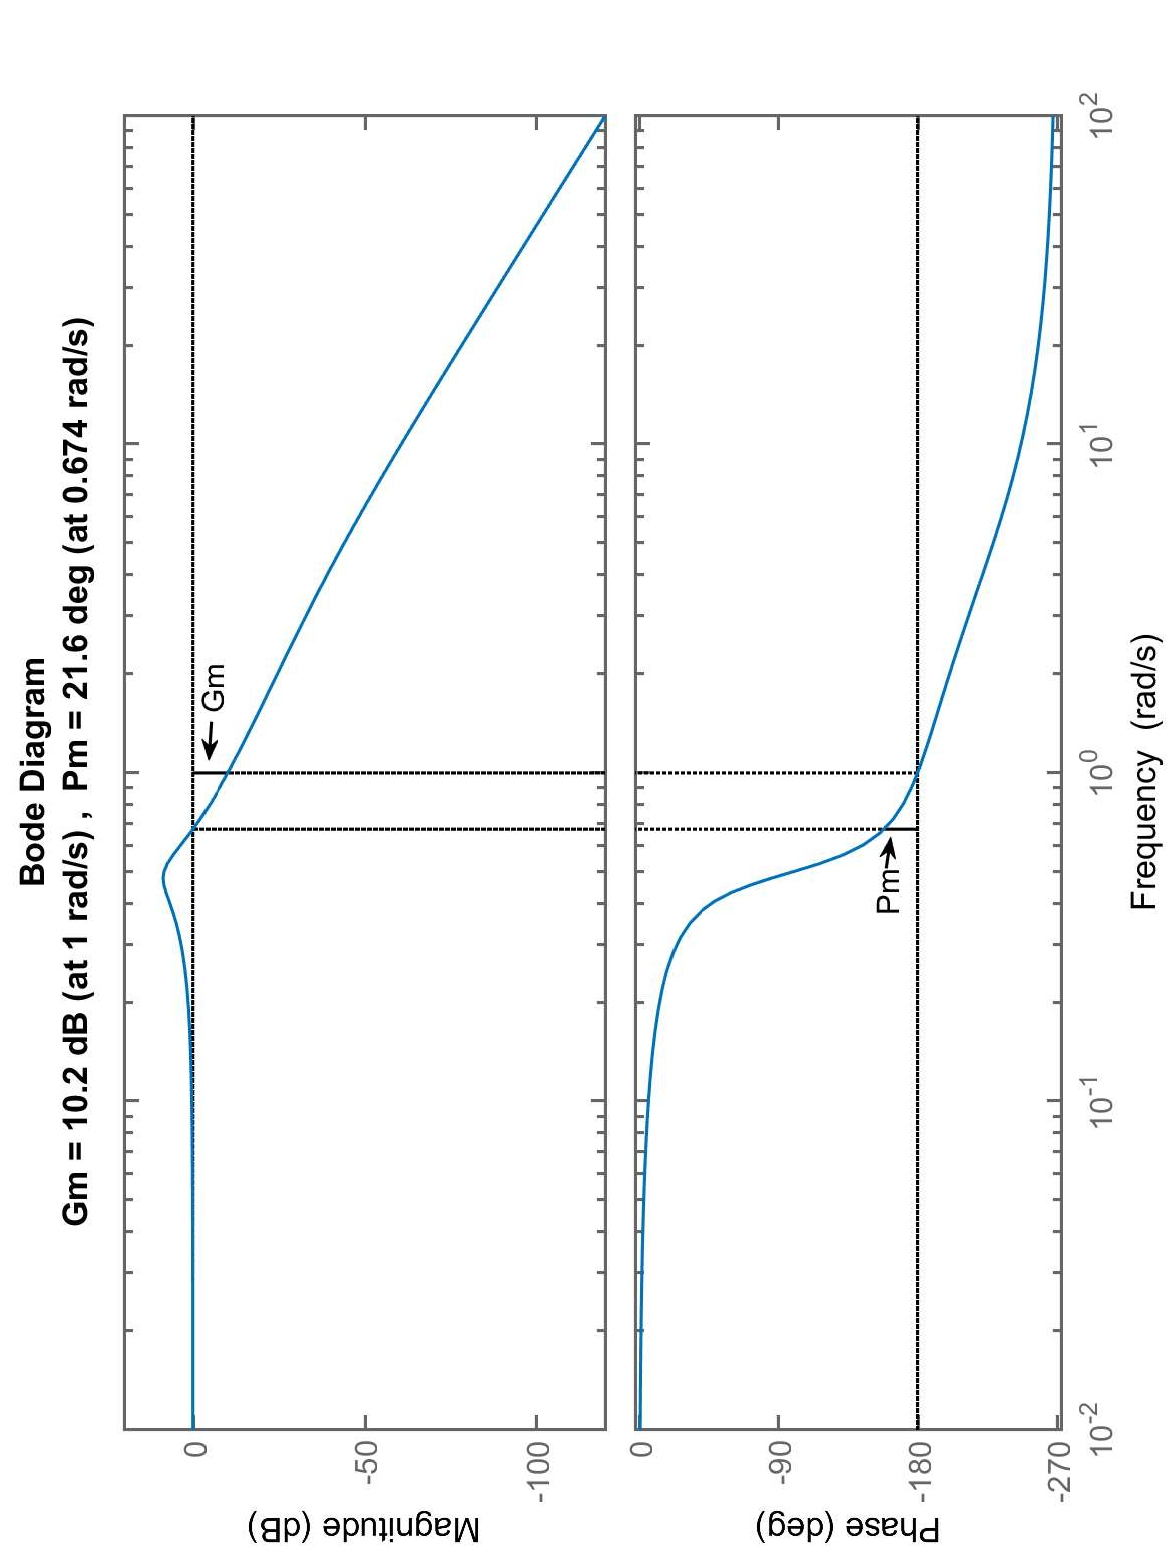
\includegraphics[width=0.6\textwidth, angle=-90]{figures/PM_GM.pdf}
\caption{Bodeplots of an open loop illustrating PM and GM.}
\label{fig:phaseGain}
\end{figure}
The phase margin is found by reading the angle velocity from the magnitude bode plot at gain = 0 dB, and finding the phase angle at this anglular velocity on the phase angle plot. The phase angle subtracted from $-180\degree$ yields the PM \citep{sou:MC}.

The gain margin is found by reading the angular velocity from the phase angle plot at the phase of $-180\degree$, and finding the gain at this angular velocity on the magnitude plot. The difference between this gain and unity gain (0 dB) is the gain margin.

From \autoref{fig:phaseGain}, it can be concluded that the phase margin is defined as how much additional phase shift it would take before the system becomes unstable. On the other hand, the gain margin describes how much the gain may change before the system becomes unstable.

In the beginning of this section, it was stated that the purpose with PM and GM is to keep uncertainties from making the system unstable. In this context, uncertainties being everything that causes the closed loop system to not behave ideally, such as circuit component sensitivity, delay caused by sampling etc. The scale of these inconsistencies is not yet know, so the exact influence these will have on the system cannot be determined. A rule of thumb regarding the PM and GM, states that PM should be greater than or equal to $45\degree$ whereas GM should be greater than or equal to 6 dB \citep{sou:PmGm}. However, to fulfill the time domain requirements, it is necessary to have $\zeta \geq 0.8$, which, based in \autoref{zeta}, results in a phase margin requirement of at least $80 \degree$.\\
From the above considerations, a list of specific requirements can now be set.